%%%%%%%%%%%%%%%%%%%%%%%%%%%%%%%%%%%%%%%%%%%%%%%%%%%%%%%%%%%%%%%%%%%%%%%%%%%%%%%%%%%%%%%%%%%
%% Ultimas modificacoes, 06/02/2012 - Alexandre Duarte 
%% Baseado no modelo latex de Isaac Maia (COPIN/UFCG)
%%
%% Para utilizar ese modelo sao necessarios os seguintes arquivos:
%%
%% ppgi.cls
%% ppgi.sty
%% mestre.sty
%%
%%
%% Mais detalhes sobre normas ABNT no latex, consultar http://abntex.codigolivre.org.br
%% Wiki interessante com dicas uteis sobre latex : http://www.tex-br.org
%%
%%
%% Para compilar esse arquivo, e' sempre importante fazer duas passagens com latex
%%%%
%%%%%%%%%%%%%%%%%%%%%%%%%%%%%%%%%%%%%%%%%%%%%%%%%%%%%%%%%%%%%%%%%%%%%%%%%%%%%%%%%%%%%%%%%%%

\documentclass[a4paper,titlepage]{ppgi}
\usepackage[portuges,english]{babel}
\usepackage{ppgi,prop,epsfig}
\usepackage{times}
\usepackage[final]{pdfpages}
\usepackage{hyperref}
\hypersetup{
    bookmarks=true,   
    pdftitle={Modelo LaTeX para Dissertações de Mestrado no Programa de Pós-Graduação em Informática da UFPB},
    pdfauthor={Alexandre Nóbrega Duarte}, 
    pdfsubject={Modelo de Documento Científico},
    pdfkeywords={Dissertação, Mestrado, PPGI, UFPB, modelo}, 
    colorlinks=true,
    linkcolor=black,
    citecolor=black,
    filecolor=black,
    urlcolor=black
 }


%-------------------------- Para usar acentuacaoo em sistemas ISO8859-1 ------------------------------------
% Se estiver usando o Microsoft Windows ou linux com essa codificacao, descomente essas linhas abaixo
% e comente as linhas referentes ao UTF8
%\usepackage[applemac]{inputenc} % Usar acentuacao em sistemas
                                % ISO8859-1, comentar a linha com
                                % \usepackage[utf8x]{inputenc}
%-----------------------------------------------------------------------------------------------------

%-------------------------- Para usar acentuacao em sistemas UTF8 ------------------------------------
% Para a maior parte das distribuicoes linux, usar essa opcao
\usepackage{ucs}
\usepackage[utf8x]{inputenc}
\usepackage[T1]{fontenc}
%-----------------------------------------------------------------------------------------------------
\usepackage{float}      
\usepackage{fancyvrb}
\usepackage{fancyheadings}
\usepackage{graphicx}
\usepackage{longtable} %tabelas longas, para tabelas que ultrapassam uma pagina
%\input{psfig.sty}
% ----------------- Para inserir codigo fonte de linguagens de programacao no documento -------------
\usepackage{listings}
\lstset{numbers=left,
stepnumber=1,
firstnumber=1,
numberstyle=\scriptsize,
extendedchars=true,
breaklines=true,
frame=tb,
basicstyle=\scriptsize,
stringstyle=\ttfamily,
showstringspaces=false
}
\renewcommand{\lstlistingname}{C\'odigo Fonte}
\renewcommand{\lstlistlistingname}{Lista de C\'odigos Fonte}

% ---------------------------------------------------------------------------------------------------

\selectlanguage{portuges}
\sloppy



\begin{document}


%%%%%%%%%%%%%%%%%%%%%%%%%%%%%%%%%%%%%%%%%%%%%%%%%%%%%%%%%%%%%%%%%%%%%%%%%%%%%%%%
\Titulo{Modelo LaTeX para Dissertações de Mestrado no Programa de Pós-Graduação em Informática da UFPB}
\Autor{Alexandre Nóbrega Duarte}
\Data{06 de Março de 2012}
\Area{Ciência da Computação}
\Pesquisa{Computação Distribuída | Sinais, Sistemas Digitais e Gráficos}
\Orientadores{O nome do seu orientador\\ (Orientador)}

\newpage
\cleardoublepage

\PaginadeRosto

\newpage
\cleardoublepage

%%%%%%%%%%%%%%%%%%%%%%%%%%%%%%%%%%%%%%%%%%%%%%%%%%%%%%%%%%%%%%%%%%%%%%%%%%%%%%%%
\begin{resumo} 
Vestibulum varius accumsan odio malesuada gravida. Duis a erat et arcu tincidunt semper sed et quam. Sed mattis semper quam vel imperdiet. Etiam tortor orci, ullamcorper ac aliquam eu, interdum quis justo. Morbi lacinia ligula ac nibh imperdiet semper. Aliquam varius tristique nisl, in blandit tellus ultrices et. Nullam est nisl, pretium sit amet vehicula quis, cursus at enim.
\\
\\
\textbf{Palavras-chave:} Palavras, chave, para, seu, trabalho.

\end{resumo}
%\newpage
\cleardoublepage

%%%%%%%%%%%%%%%%%%%%%%%%%%%%%%%%%%%%%%%%%%%%%%%%%%%%%%%%%%%%%%%%%%%%%%%%%%%%%%%%
\begin{summary}
Vestibulum varius accumsan odio malesuada gravida. Duis a erat et arcu tincidunt semper sed et quam. Sed mattis semper quam vel imperdiet. Etiam tortor orci, ullamcorper ac aliquam eu, interdum quis justo. Morbi lacinia ligula ac nibh imperdiet semper. Aliquam varius tristique nisl, in blandit tellus ultrices et. Nullam est nisl, pretium sit amet vehicula quis, cursus at enim.
s\\ 
\\
\textbf{Keywords:} Keywords, for, your, work, (in, english, please)
\end{summary}

%\newpage
\cleardoublepage

%%%%%%%%%%%%%%%%%%%%%%%%%%%%%%%%%%%%%%%%%%%%%%%%%%%%%%%%%%%%%%%%%%%%%%%%%%%%%%%%
%% Definicao do cabecalho: secao do lado esquerdo e numero da pagina do lado direito
\pagestyle{fancy}
\addtolength{\headwidth}{\marginparsep}\addtolength{\headwidth}{\marginparwidth}\headwidth = \textwidth
\renewcommand{\chaptermark}[1]{\markboth{#1}{}}
\renewcommand{\sectionmark}[1]{\markright{\thesection\ #1}}\lhead[\fancyplain{}{\bfseries\thepage}]%
	     {\fancyplain{}{\emph{\rightmark}}}\rhead[\fancyplain{}{\bfseries\leftmark}]%
             {\fancyplain{}{\bfseries\thepage}}\cfoot{}

%%%%%%%%%%%%%%%%%%%%%%%%%%%%%%%%%%%%%%%%%%%%%%%%%%%%%%%%%%%%%%%%%%%%%%%%%%%%%%%%
\selectlanguage{portuges}

\Sumario
\ListadeSimbolos
\listoffigures
\listoftables
\lstlistoflistings %lista de codigos fonte - Para inserir a listagem de
% codigos fonte

\newpage
\cleardoublepage
\Introducao


%%%%%%%%%%%%%%%%%%%%%%%%%%%%%%%%%%%%%%%%%%%%%%%%%%%%%%%%%%%%%%%%%%%%%%%%%%%%%%%%
%
% Hifenizacao - Colocar lista de palavras que nao devem ser separadas e que 
% nao estao no dicionario portugues.
% As palavras do dicionario portugues ja sao separadas corretamente pelo lateX
%
\hyphenation{ gLite OurGrid GridDoctor }


%%%%%%%%%%%%%%%%%%%%%%%%%%%%%%%%%%%%%%%%%%%%%%%%%%%%%%%%%%%%%%%%%%%%%%%%%%%%%%%%
%% A partir daqui coloque seus capitulos. Sugere-se que eles sejam inseridos com o comando \input
%% Da seguinte maneira:
%% 
\chapter{Introdução} \label{intro}

\lstset{language=Java}
\lstinputlisting[caption=Exemplo de como inserir um arquivo com c妖igo fonte,
label=code:Parser.java] {code/Parser.java}

\begin{figure}
\centering
\caption{Exemplo de como inserir uma figura}\label{fig:eela}
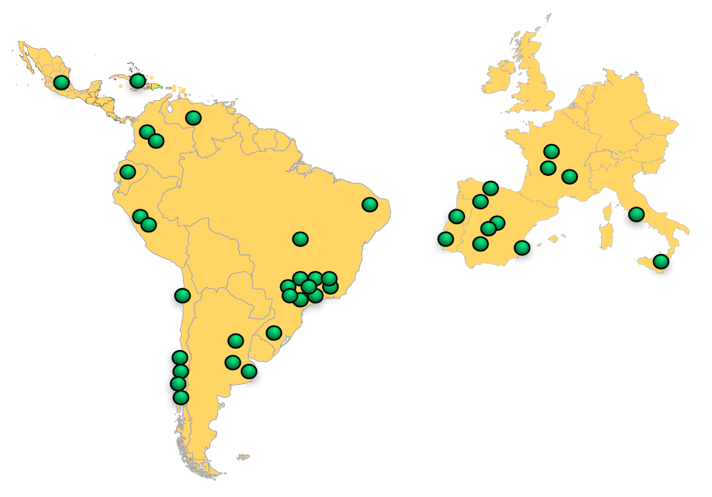
\includegraphics[width=0.7\textwidth]{images/eela.png}
\end{figure}


\begin{table}
\centering
\caption{Exemplo de como inserir uma tabela}\label{tab:exp-app}
\begin{tabular}{ | l | c | c | c |}\hline
 				   & Falha App. & Falha SE & Falha CE\\\hline
Resultado Esperado & 1.052       & 0        & 0       \\\hline 
Resultado Obtido   & 1.052       & 0        & 0       \\\hline 
Resultado Real  & 991        & 37       & 24      \\\hline 
\end{tabular}
\end{table}


\section{Motivação}\label{sec:motiva}

Aqui vai um exemplo de como citar uma refer刃cia contida no arquivo main.bib \cite{nakada2007job}.

\section{Objetivos}

\subsection{Objetivo Geral}

\subsection{Objetivos Especificos}

\section{Metodologia}

\section{Publicações Relacionadas}

\section{Estrutura da Dissertação}
%\chapter{Fundamentação Teórica}\label{cap:fundamentacao}

\section{Assunto abordado 1}

\section{Assunto abordado 2}

\section{Considerações Finais}






%\chapter{Trabalhos Relacionados}\label{cap:relacionados}


\section{Trabalhos relacionados sobre o tema X}
\subsection{Discussão}

\section{Trabalhos relacionados sobre o tema Y}
\subsection{Discussão}

\section{Consideraõees Finais}
%\chapter{Proposta de dissertação}\label{cap:miolo}


\section{Sessão 1 sobre o seu trabalho}

\section{Sessão 2 sobre o seu trabalho}

\section{Considerações Finais}

%\chapter{Proposta de Avaliação Experimental}\label{cap:avalia}

\section{Proposta de Estudo de Caso}

\subsection{Ferramentas e Tecnologia}
\subsection{Requisitos}
\subsection{Planejamento de Execução}

\section{Proposta de Experimento}

\subsection{Plano do Experimento}
\subsection{Planejamento de Execução}

\section{Considerações Finais}



%\chapter{Conclusão e Cronograma}\label{cap:conclusao}




%%%%%%%%%%%%%%%%%%%%%%%%%%%%%%%%%%%%%%%%%%%%%%%%%%%%%%%%%%%%%%%%%%%%%%%%%%%%%%%%
%% BIbliografia
%% Coloque suas referencias no arquivo ref.bib

\bibliographystyle{abnt-alf} % estilo de bibliografia   plain,unsrt,alpha,abbrv.
\bibliography{main} % arquivos com as entradas bib.

%Faz aparecer a referencia bibliografica no indice
\addcontentsline{toc}{section}{\numberline{}Referências Bibliográficas}

%%%%%%%%%%%%%%%%%%%%%%%%%%%%%%%%%%%%%%%%%%%%%%%%%%%%%%%%%%%%%%%%%%%%%%%%%%%%%%%%
%% Apendice
% Caso seja necessario algum apendice

\appendix
%\chapter{Apêndice A}}\label{apendice-a}

%\chapter{Apêndice B}}\label{apendice-b}

%\chapter{Apêndice C}}\label{apendice-c}

%\chapter{Apêndice D}}\label{apendice-d}

%%%%%%%%%%%%%%%%%%%%%%%%%%%%%%%%%%%%%%%%%%%%%%%%%%%%%%%%%%%%%%%%%%%%%%%%%%%%%%%%

\end{document}
